\documentclass[11pt,a4paper]{amsart}
\usepackage[utf8]{inputenc}
\usepackage[icelandic]{babel}
\usepackage[T1]{fontenc}
\usepackage{amsmath, amsthm, amssymb, amsfonts}
\usepackage{enumerate}
\usepackage{graphicx}
\usepackage{fancyhdr}
\usepackage{booktabs}
\usepackage{float}
\usepackage{hyperref}
\usepackage{caption}
\usepackage{subcaption}
\usepackage{setspace} 
\onehalfspacing
\addtolength{\textheight}{2.4cm}
\addtolength{\hoffset}{-1.2cm}
\addtolength{\voffset}{-2cm}
\addtolength{\textwidth}{2.3cm}

% Define new commands and operators
\newcommand{\N}{\mathbb{N}}
\newcommand{\No}{\N_0}
\newcommand{\Z}{\mathbb{Z}}
\newcommand{\perms}{\mathfrak{S}}

\DeclareMathOperator{\prst}{\mathcal{P}} 
\DeclareMathOperator{\rem}{rem}	
\DeclareMathOperator{\id}{id}
% End of new commands definitions

% Setup theorem styles
\theoremstyle{plain}
\newtheorem{theorem}{Theorem}[section]
\newtheorem{proposition}[theorem]{Proposition}
\newtheorem{lemma}[theorem]{Lemma}
\newtheorem{corollary}[theorem]{Corollary}
\newtheorem{conjecture}[theorem]{Conjecture}

\theoremstyle{definition}
\newtheorem{definition}[theorem]{Definition}
\newtheorem{example}[theorem]{Example}

\theoremstyle{remark}
\newtheorem*{remark}{Remark}
% End of theorem styles setup

% Single spacing after dots and colons
\frenchspacing

\begin{document}

\title{Hópaverkefni 1 \\ Áhrif Iceland Airwaves á gistinætur}
\authors{Arnar Ingi Halldórsson, Halldór Stefánsson, Hjörleifur G. Bergsteinsson, Lárus Ívar Ívarsson og Þór Tómasarson}
\address{School of Computer Science, Reykjavik University,
Menntavegi 1, \newline 101 \mbox{Reykjavík}, Iceland}
\date{\today}

\maketitle

Í þessu verkefni er okkur ætlað að skoða hvaða áhrif tónlistarhátíðin Iceland Airwaves hefur á gistinætur.\par
Til að byrja með getur notandinn annað hvort valið "Data Type 1" eða "Data Type 2" í notendaviðmótinu(mynd~\ref{fig:noten}), data1 er sjálfgefið með núverandi gögnum en í data2 getur notandinn set sýna eigin skrá t.d. ef notandinn vill skoðað sambærilega gögn eftir ár, þá setur hann skránna þar inn. Síðan getur notandinn valið hvaða gögn hann vill skoða.\\\par

Í myndum~\ref{fig:mynd2} og ~\ref{fig:mynd3} notum við aðferð minnstu kvaðrótar til þess að fá jöfnu bestu línu, til að hjálpa okkur til að spá áframhaldinu. Jafnan fyrir íslenskar gistinætur er $$ y = 1077.9 \cdot x - 2139441.4  $$ og fyrir útlendinga $$ y = 4532.5 \cdot x - 9023834.1 $$
Okkar spá fyrir 2014 er þá að fjöldi gistinótta hjá íslendingum verður 31435 gistingar og hjá útlendingum 104650 gistingar.

Við sjáum á myndum~\ref{fig:mynd4} og ~\ref{fig:gist_spa} getum við lesið hvernig við teljum að október og nóvember hefðu þróast með Airwaves hjá íslendingum og útlendingum miðað við raunþróun. Spáinn miðast við september, þar sem við notum okkur þróunin þar, notast er við september vegna þess þar er engin stórviðburður sem gæti haft áhrif á tölurnar. Hjá íslendingum sjáum við að gistingin byrjar að aukast eftir 2003 miðað við spár bæði í október og nóvember og þar sem Airwaves var haldið í október fram að 2012 er getum við ekki rekið þessa aukningar vegna Airwaves. Hjá útlendingum sjáum við einnig aukningu í október miðað við spá alveg aftur til 1999, sem aukist hefur jafn og þétt. Við getum gert ráð fyrir að Airwaves hafi áhrif á útlendingum frá og með 2012, því þá er hátíðin haldin í nóvember og gistingar aukast augljóslega.

Út frá mynd~\ref{fig:gist_hlutf} sjáum að til ársins 2012 er lækkun á gistinóttum frá október til nóvember, en á þeim tíma var Airwaves í október. Árið 2012 og eftir það er Airwaves hins vegar haldið í nóvember og þá breytist hallatalan ekki eins mikið á milli október og nóvember.\par

Undanfarin ár hefur verið mikil aukning í ferðamönnum hér á landi eins og sést þegar gögnin eru skoðuð og því erfitt að meta hversu mikil áhrif Airwaves hefur á aukninguna. Þó teljum við um aukningu á gistinóttum sé að ræða vegna Airwaves og sést það aðallega á mynd~\ref{fig:gist_spa}, þegar hátíðin er haldin í nóvember og fjöldi gistinótt eykst augljóslega miðað við árin á undan.

\section{Appendix}

\begin{figure}[H]
	\centering
	\begin{subfigure}[b]{0.4\textwidth}
		\includegraphics[height=40mm]{mynd2.png}
		\caption{$ Least\ square\ 1$\label{fig:mynd2}}
	\end{subfigure}
	\begin{subfigure}[b]{0.4\textwidth}
		\includegraphics[height=40mm]{mynd3.png}
		\caption{$ Least\ square\ 2 $\label{fig:mynd3}}	
	\end{subfigure}
\end{figure}

\begin{figure}[H]
	\centering
	\begin{subfigure}[b]{0.45\textwidth}
		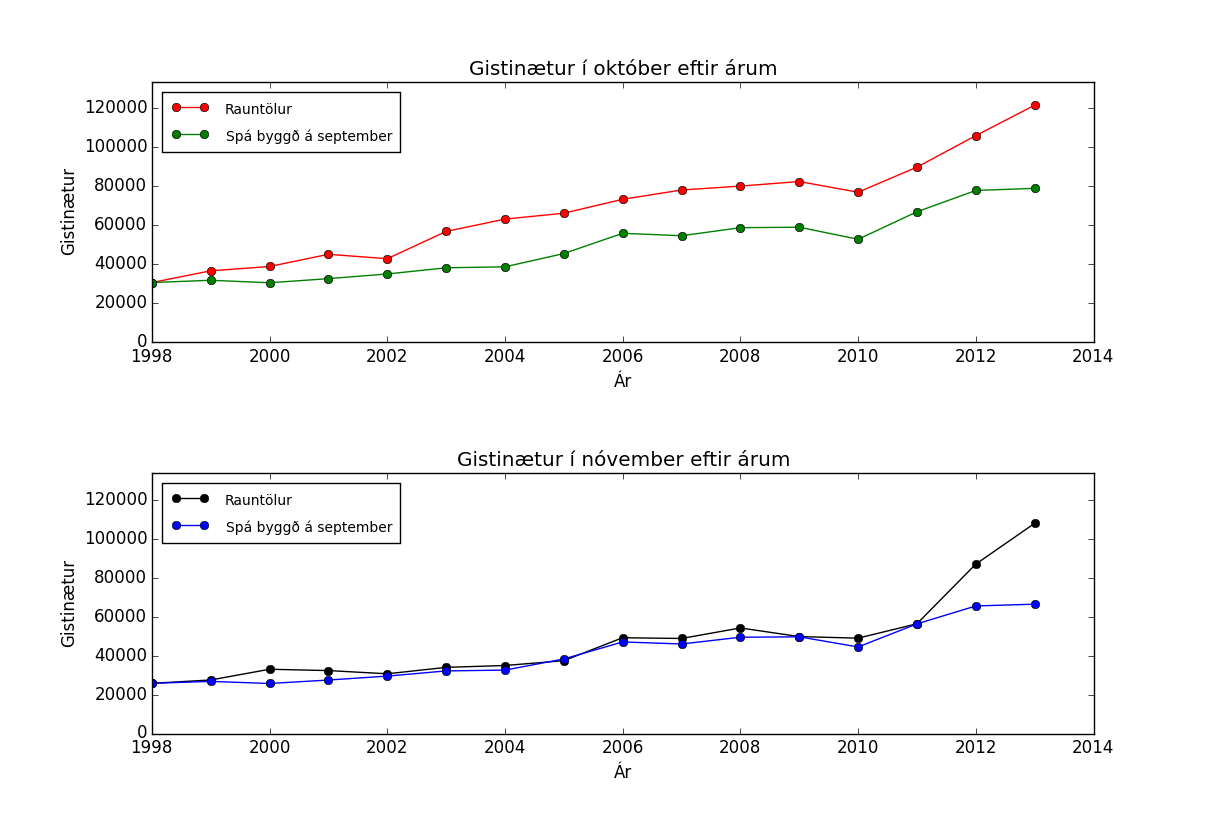
\includegraphics[height=40mm]{figure_3.png}
		\caption{$ Rauntolur\ og\ spar\ a\ gistinottum $\label{fig:mynd4}}
	\end{subfigure}
	\begin{subfigure}[b]{0.45\textwidth}
		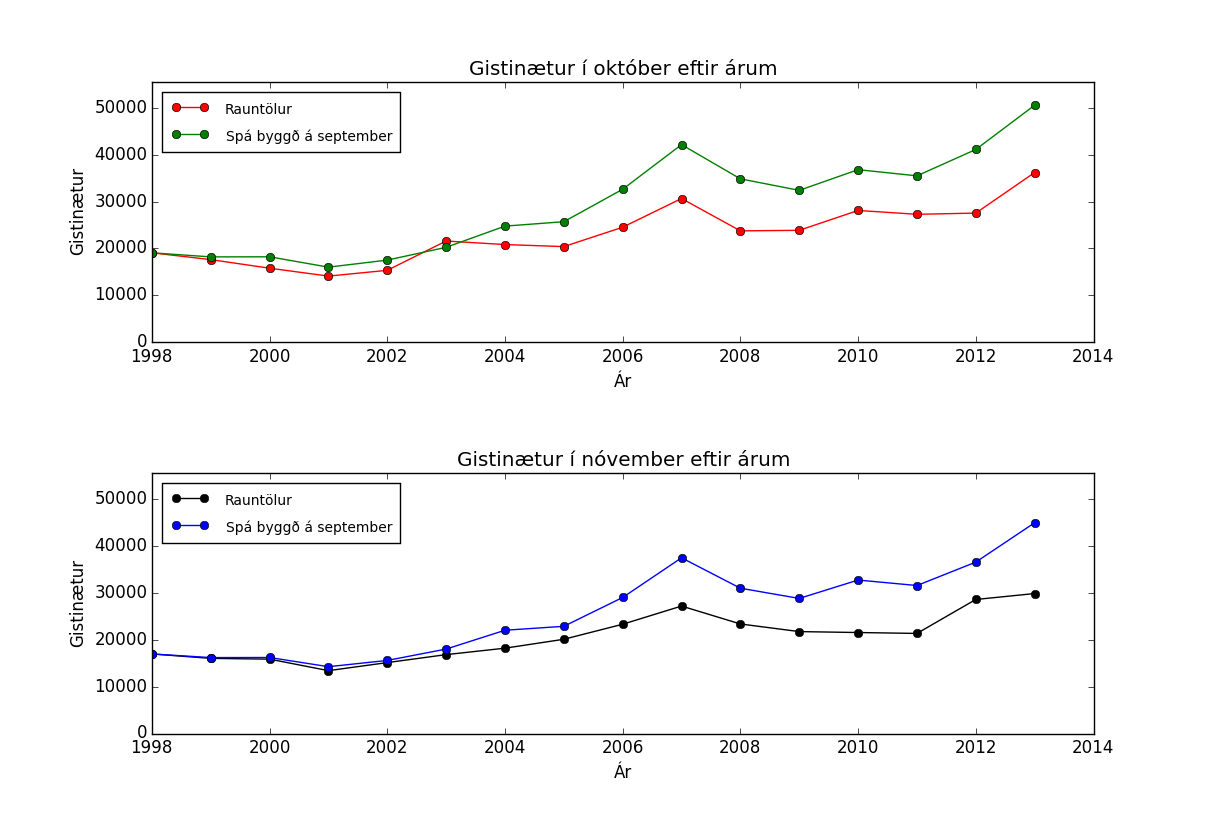
\includegraphics[height=40mm]{figure_2.png}
		\caption{$ Rauntolur\ og\ spar\ a\ gistinottum $\label{fig:gist_spa}}
	\end{subfigure}
\end{figure}

\begin{figure}[H]
\centering
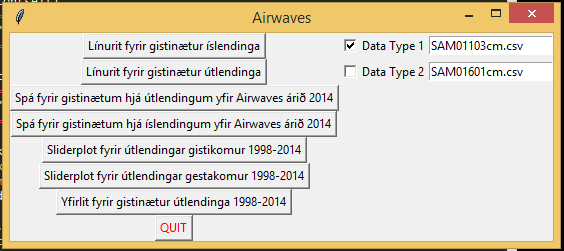
\includegraphics[height=30mm]{GUI.png}
\caption{$ Notendavidmot $\label{fig:noten}}
\end{figure}

\begin{figure}[H]
\centering
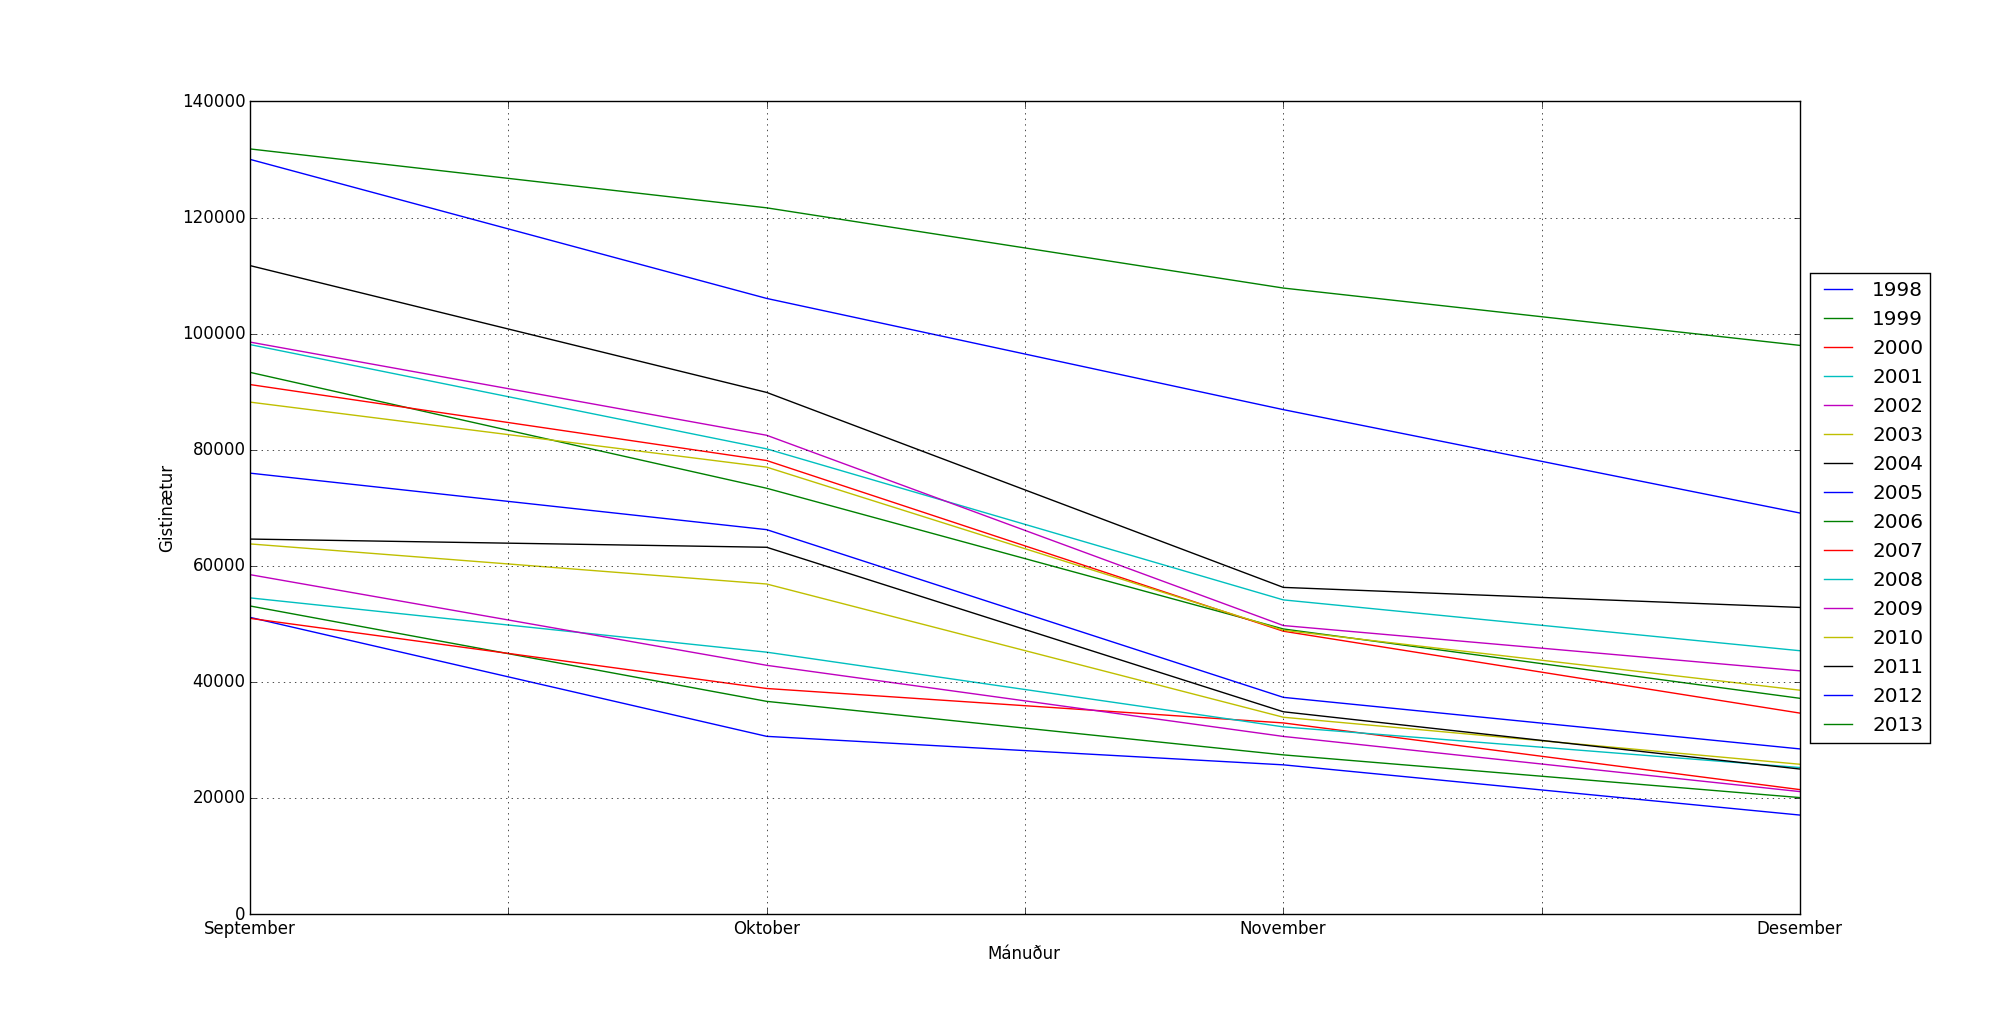
\includegraphics[height=30mm]{my_plot.png}
\caption{$ Gistinaetur\ manuda\ i\ kringum\ Iceland\ Airwaves $\label{fig:gist_hlutf}}
\end{figure}
	
\bibliography{citations}{}
\bibliographystyle{plain}
\end{document}